\documentclass[../psets.tex]{subfiles}

\pagestyle{main}
\renewcommand{\leftmark}{Problem Set \thesection}
\stepcounter{section}

\begin{document}




\section{Cycles, Cubes, and the Dodecahedron}
\begin{enumerate}
    \item \marginnote{10/10:}If $\sigma$ is an element of $S_n$, then $\sigma$ has a cycle decomposition into disjoint cycles of various lengths (let us include 1-cycles). Since disjoint cycles commute, the shape of the element is determined by the lengths of the various cycles, which we can assume are put in decreasing order. Any two elements with the same cycle shape are conjugate, so the conjugacy classes are determined by writing $n$ ($=52$, say) as a sum of decreasing integers.
    \begin{enumerate}
        \item Find the conjugacy class in $S_{52}$ with the largest number of elements.
        \item Find the conjugacy class in $S_{52}$ which contains the element of largest order.
    \end{enumerate}
    \item Let $k\leq n$ be even. Prove that every element in $S_n$ can be written as a product of $k$-cycles.
    \item Let $D$ be a regular dodecahedron. You may assume for this question that it is possible to inscribe a cube $C$ on the vertices of $D$ as shown below.
    \begin{center}
        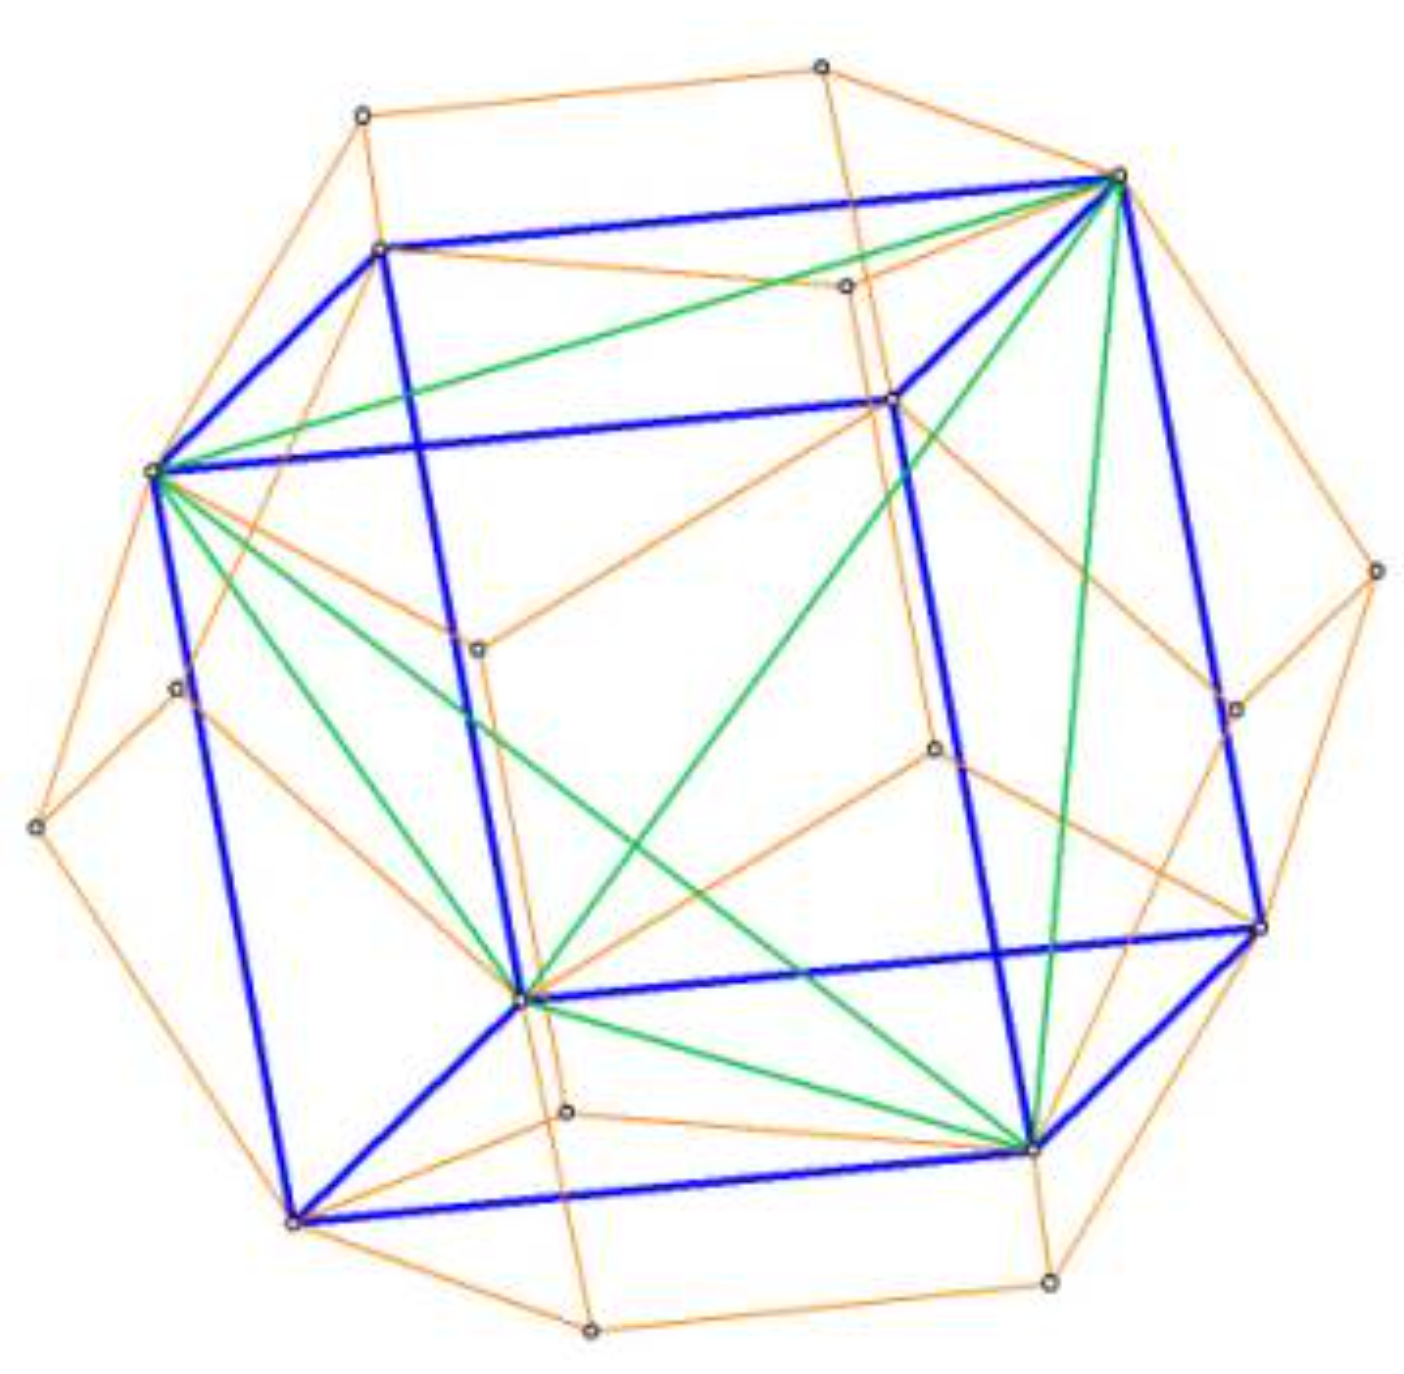
\includegraphics[width=0.4\linewidth]{../ExtFiles/dodecahedronCube.png}
    \end{center}
    \emph{Remember the following important distinction}: An object $X$ in $\R^3$ is \textbf{fixed pointwise} by $g$ if every point on $X$ is fixed by $g$, that is, if $gx=x$ for all $x\in X$. An object $X\in\R^3$ is \textbf{preserved} by $g$ if every point on $X$ maps to another (possibly different) point on $X$, i.e., for all $x\in X$, there exists $y\in X$ such that $gx=y$. As an example, the circle centered at the origin is preserved by any rotation through the origin, but is not fixed pointwise unless the rotation is trivial.
    \begin{itemize}
        \item If $F$ is a face, call a line between two vertices of $F$ an \textbf{internal line} if the vertices are not adjacent. That is, an internal line is a line between two vertices of a pentagonal face which is not an edge of the pentagon.
        \item Observe that the cube $C$ has 12 edges, and that each edge lies on exactly one of the 12 faces of $D$ as an internal line.
        \item Choose a face $F$ of $D$ and let $g$ be the symmetry of $D$ of order 5 which is a rotation by $2\pi/5$ through the line passing through the middle of $F$ and the middle of the opposite face $-F$.
    \end{itemize}
    \begin{enumerate}
        \item Label the vertices of a face $F$ from 1 to 5. Suppose that $C=C_{(1,3)}$ intersects $F$ in the internal edge from 1 to 3.
        \item Show that for any such $g$, the five cubes $C_{(1,3)}$, $C_{(2,4)}$, $C_{(3,5)}$, $C_{(1,4)}$, and $C_{(2,5)}$ obtained by applying the powers of $g$ to each cube are distinct because they intersect $F$ in different internal lines (which are the lines between vertices indicated by the notation).
        \item Show that \emph{any} symmetry of $D$ takes $C$ to one of these five cubes. Hint: Any pair of cubes share two vertices $\mathbf{v},\mathbf{w}$ on $F$ lying on an internal line of $F$ which are connected by an edge of the cube. Given a cube centered at the origin with vertices $\mathbf{v},\mathbf{w}$ and $|\mathbf{v}|=|\mathbf{w}|$ connected by an edge, show that the eight vertices of the cube are
        \begin{equation*}
            \pm\mathbf{v},\ \pm\mathbf{w},\ \pm\mathbf{u},\ \pm\left( \frac{\mathbf{v}-\mathbf{w}}{2} \right)
        \end{equation*}
        where $\mathbf{u}$ is the (unique up to a $\pm$ sign) vector with $|\mathbf{u}|=|\mathbf{v}|=|\mathbf{w}|$ and $\mathbf{u}\cdot\mathbf{v}=\mathbf{u}\cdot\mathbf{w}=0$.
        \item Let $\mathbf{v}_i$ indicate the vector corresponding to edge $i$ of $F$. Deduce that there are exactly two cubes which have $\mathbf{v}_i$ as a vertex, and that the only vertices that these two cubes have in common are $\pm\mathbf{v}_i$.
        \item (*) Show that any rigid motion of $D$ (i.e., any element of $\text{SO}(3)$ preserving $D$) permutes the 5 cubes. Hint: Show that if a symmetry $\sigma$ preserves the two cubes passing through $\mathbf{v}_i$, then it preserves their intersection and deduce that
        \begin{equation*}
            \sigma\mathbf{v}_i = \pm\mathbf{v}_i
        \end{equation*}
        Deduce that this identity must hold for every $i$, and use this (and HW1) to show that this implies that $\sigma$ is the identity.
        \item Deduce that the symmetry group of the dodecahedron is a subgroup of $S_5$ of order 60.
    \end{enumerate}
    \item Embed the cube inside $\R^3$ so that the centers of each face are at
    \begin{align*}
        A &= (1,0,0)&
        B &= (-1,0,0)&
        C &= (0,1,0)&
        D &= (0,-1,0)&
        E &= (0,0,1)&
        F &= (0,0,-1)
    \end{align*}
    Considering the symmetry group of $C$ as a subgroup of $\text{SO}(3)$, write down the matrix of $\text{SO}(3)$ corresponding to the following elements.
    \begin{enumerate}
        \item $\sigma=(A,C,E)(B,D,F)$.
        \item $\tau=(C,E,D,F)$.
        \item $\sigma\tau=(A,C,E)(B,D,F)(C,E,D,F)=(A,C)(B,D)(E,F)$.
    \end{enumerate}
\end{enumerate}




\end{document}